\clearpage
\setcounter{section}{4}
\section{Complete metric spaces}

\topic{Completeness and closed subspaces}
\begin{note}{Completeness is a property of the metric}
A metric space is complete if every Cauchy sequence has a limit in the space. A subset is complete when equipped with the inherited metric.

$\R$, $\C$, finite-dimensional $\ell^p$ spaces, and every discrete space are complete. $(0,1)$ and $[0,1)$ with the usual metric are incomplete: a sequence can approach an excluded endpoint. $\Q$ is incomplete: rational approximations to $\sqrt2$ are Cauchy but have no rational limit.

Completeness is preserved under bi-Lipschitz maps and Cauchy-equivalent metrics. It is not preserved by arbitrary homeomorphisms: $(\R,d_{NS})$ is homeomorphic to usual $\R$ but incomplete because $n$ is Cauchy and cannot converge to a finite real in $d_{NS}$.
\end{note}
\begin{method}{The closed-subset shortcut}
A complete subset of \emph{any} metric space is closed. A closed subset of a \emph{complete} metric space is complete. Thus, when the ambient space is complete, subset completeness is equivalent to closedness. In particular a subset of usual $\R^n$ is complete iff it is closed, without needing boundedness.

To prove incompleteness construct a Cauchy sequence with a missing limit. It is usually easiest to find its limit in a larger known complete space and use uniqueness to exclude any alternative limit in your space.
\end{method}
\begin{exam}{2025 Q4(a): complete iff closed in a complete ambient space}
Let $E$ be complete and $A\subseteq E$. Prove that $A$ is complete iff it is closed in $E$.
\end{exam}
\begin{answer}
Suppose $A$ is complete. Let $a_n\in A$ with $a_n\to p$ in $E$. Then $(a_n)$ is Cauchy in $E$ and hence in the subspace $A$. By completeness of $A$, $a_n\to a$ for some $a\in A$. This is also convergence in $E$, so uniqueness gives $p=a\in A$. Hence $A$ is closed.

Conversely, suppose $A$ is closed and let $(a_n)$ be Cauchy in $A$. It is Cauchy in $E$, so by completeness of $E$ there is $p\in E$ with $a_n\to p$. Since $A$ is closed, $p\in A$. Thus the sequence converges in $A$, proving completeness.
\end{answer}
\begin{exam}{2022 Q3(b): uniform continuity and completeness}
Let $f:E\to E'$ be a homeomorphism, with $f$ uniformly continuous and $E'$ complete. Prove that $E$ is complete.
\end{exam}
\begin{answer}
Let $(x_n)$ be Cauchy in $E$. Uniform continuity sends Cauchy sequences to Cauchy sequences: for any target tolerance choose one $\delta$ valid for all pairs, then apply Cauchyness in $E$. Thus $(f(x_n))$ is Cauchy in $E'$, and completeness gives $f(x_n)\to y\in E'$. Since $f^{-1}$ is continuous, $x_n=f^{-1}(f(x_n))\to f^{-1}(y)\in E$. Therefore $E$ is complete.

Notice the direction: uniform continuity is needed for $f$ to send the original Cauchy sequence forward, and continuity of $f^{-1}$ brings its limit back.
\end{answer}


\topic{Completeness of function spaces and uniform limits}
\begin{note}{Why the sup metric is uniform convergence}
$d_{\sup}(f_n,f)\to0$ iff
\[\forall\varepsilon>0\ \exists N\ \forall n\ge N\ \forall s\in S:\ d_E(f_n(s),f(s))<\varepsilon.\]
The index $N$ works for every input. Pointwise convergence allows $N$ to depend on the input and is weaker. For instance $f_n(t)=t^n$ on $[0,1]$ converges pointwise to a function which is $0$ below $1$ and $1$ at $1$, but this limit is discontinuous, so the convergence cannot be uniform.
\end{note}
\begin{method}{Prove $\ell^\infty(S;E)$ complete}
Assume $E$ complete. Start with an arbitrary sup-Cauchy sequence $(f_n)$. For each $s$, $d_E(f_n(s),f_m(s))\le d_{\sup}(f_n,f_m)$, so define $f(s)=\lim_n f_n(s)$ using completeness of $E$. Next pass $m\to\infty$ in a \emph{uniform} Cauchy bound; this gives uniform convergence. Finally prove $f$ bounded by comparing it to a fixed bounded $f_N$. Both membership and convergence must be checked.
\end{method}
\begin{exam}{2023 Q3(b), 2024 Q3(d): completeness of the sup space}
Let $E$ be complete. Prove $\ell^\infty(S;E)$ is complete.
\end{exam}
\begin{answer}
Let $(f_n)$ be Cauchy in the sup metric. For every $s\in S$, $(f_n(s))$ is Cauchy in $E$, so define $f(s)=\lim_n f_n(s)$. Given $\varepsilon>0$, choose $N$ such that $d_{\sup}(f_n,f_m)<\varepsilon/2$ for $n,m\ge N$. For any $s$ and $n\ge N$, let $m\to\infty$ to obtain
\[d_E(f_n(s),f(s))\le\varepsilon/2.\]
Taking the supremum gives $d_{\sup}(f_n,f)\le\varepsilon/2<\varepsilon$, once $f$ is known to belong to the space.

For membership, use the preceding estimate with tolerance $2$ to choose a fixed $N_0$ for which $d_E(f_{N_0}(s),f(s))\le1$ for every $s$. For $s,t\in S$,
\[d_E(f(s),f(t))\le1+d_E(f_{N_0}(s),f_{N_0}(t))+1\le2+\diam f_{N_0}(S).\]
Thus $f$ is bounded. It lies in $\ell^\infty(S;E)$ and $f_n\to f$ there, proving completeness. For $E=[0,1]$ every function is automatically bounded and pointwise limits stay in the complete interval, giving the 2024 special case.
\end{answer}
\begin{note}{Uniform limits of continuous maps are continuous}
Let $f_n:E\to F$ be continuous and $f_n\to f$ uniformly. Fix $p$ and $\varepsilon>0$. Choose one $N$ with $d_{\sup}(f_N,f)<\varepsilon/3$. Then continuity of this fixed $f_N$ gives $\delta>0$ such that $d_E(x,p)<\delta$ implies $d_F(f_N(x),f_N(p))<\varepsilon/3$. Therefore
\begin{align*}
d_F(f(x),f(p))&\le d_F(f(x),f_N(x))+d_F(f_N(x),f_N(p))\\
&\quad+d_F(f_N(p),f(p))<\varepsilon.
\end{align*}
Thus $C_b(E;F)$ is closed in $\ell^\infty(E;F)$, and is complete if $F$ is complete. If the domain $K$ is sequentially compact, continuous maps have bounded image, so $C(K;F)=C_b(K;F)$.
\end{note}
\begin{exam}{2025 Q4(b): completeness of continuous-function space}
Let $I=[0,1]$ and $E$ be complete. Explain why $C(I;E)\subseteq\ell^\infty(I;E)$, and prove $C(I;E)$ is complete.
\end{exam}
\begin{answer}
The interval $I$ is sequentially compact by Bolzano--Weierstrass. A continuous image of a sequentially compact space is sequentially compact, hence bounded. Thus every $f\in C(I;E)$ belongs to $\ell^\infty(I;E)$.

By the previous completeness proof, $\ell^\infty(I;E)$ is complete. If a sequence in $C(I;E)$ converges in the sup metric to $f$, its convergence is uniform. The $\varepsilon/3$ argument above proves $f$ continuous, so $C(I;E)$ is closed in the complete sup space. Therefore it is complete.
\end{answer}
\begin{tip}
In the sup-space completeness proof, pointwise convergence is only the first step. The uniform Cauchy bound is what gives uniform convergence. After passing to a limit a strict $<$ can become $\le$; starting with $\varepsilon/2$ handles this cleanly.
\end{tip}


\topic{Embedding, dense extension and completion}
\begin{note}{Embedding any metric space into a complete normed space}
For nonempty $E$ fix $\omega\in E$ and define
\[j_\omega(x)(p)=d(x,p)-d(\omega,p),\qquad p\in E.\]
The reverse triangle inequality gives $|j_\omega(x)(p)|\le d(x,\omega)$, so each function is bounded. Also
\[|j_\omega(x)(p)-j_\omega(y)(p)|=|d(x,p)-d(y,p)|\le d(x,y).\]
At $p=y$ equality holds. Hence $\norm{j_\omega(x)-j_\omega(y)}_\infty=d(x,y)$. This is an isometric embedding into the complete real normed space $\ell^\infty(E;\R)$.

For bounded $E$ one can simply use $x\mapsto(p\mapsto d(x,p))$. The reference-point subtraction is essential for unbounded $E$. The supplied notes say the embedding proof is not expected from memory, but the guided construction is useful practice.
\end{note}
\begin{note}{Extending Lipschitz maps from a dense set}
Let $A$ be dense in $E$, $F$ complete, and $f_0:A\to F$ be $L$-Lipschitz. Define $f(x)=\lim_n f_0(a_n)$ for any $a_n\in A$ tending to $x$.

Existence: $(a_n)$ is Cauchy, so $(f_0(a_n))$ is Cauchy and has a limit in $F$. Independence: if $b_n\to x$, then
\[d_F(f_0(a_n),f_0(b_n))\le L[d_E(a_n,x)+d_E(x,b_n)]\to0.\]
Thus the definition is independent of the approximating sequence. Constant sequences show extension. For $a_n\to x$, $b_n\to y$, passing to limits in the Lipschitz inequality proves $d_F(f(x),f(y))\le Ld_E(x,y)$. The optimal constant is unchanged because restricting to $A$ gives the reverse bound.

Any continuous extension must take this same value by sequential continuity, proving uniqueness. If $f_0$ is isometric the equality also passes to limits. Uniformly continuous maps extend similarly: use preservation of Cauchy sequences and choose a uniform $\delta$, with $\varepsilon/2$ margins, before taking limits.
\end{note}
\begin{exam}{Section 5 practice: dense extension and its limitation}
Show the map $f_0:\Q\to\R$, $f_0(q)=2q+1$, has a unique continuous extension to $\R$, and determine its Lipschitz constant. Explain why arbitrary continuous maps on dense subsets need not extend.
\end{exam}
\begin{answer}
For rationals $q,r$, $|f_0(q)-f_0(r)|=2|q-r|$, so $f_0$ is $2$-Lipschitz. Since $\Q$ is dense in $\R$ and the target $\R$ is complete, the extension theorem applies. For rationals $q_n\to x$,
\[f(x)=\lim_n(2q_n+1)=2x+1.\]
Its Lipschitz constant is exactly $2$, since equality holds for every distinct pair.

For failure with continuity alone, $h(x)=\sin(1/x)$ on the dense subset $\R\setminus\{0\}$ is continuous but cannot extend continuously to zero. The sequences $a_n=(\pi/2+2\pi n)^{-1}$ and $b_n=(3\pi/2+2\pi n)^{-1}$ both tend to zero but their images are constantly $1$ and $-1$ respectively.
\end{answer}
\begin{note}{Completion: definition and examples}
A completion is a complete space $\widehat E$ with an isometry $\iota:E\to\widehat E$ whose image is dense. The density condition rules out adding unrelated extra points. Examples: the completion of usual $\Q$ is $\R$; of $(0,1)$ is $[0,1]$; of $(\R,d_{NS})$ is $[-\pi/2,\pi/2]$ with embedding $\arctan$.

Every metric space has a completion: embed into a complete normed space and take the closure of the image. Two completions are uniquely related by an isometry respecting their embeddings. To see surjectivity, the extended isometry has a complete, hence closed, image containing the dense embedded copy of $E$, so its image is all of the target completion. Uniqueness follows by equality on that dense copy.

\textbf{Status:} the existence/uniqueness proof is marked non-examinable in the supplied notes. The optional $L^1$ completion of $(C(I),d_1)$ uses integrable functions modulo equality almost everywhere; ordinary pointwise functions must be quotiented because integral distance can be zero between distinct functions.
\end{note}


\topic{Banach's contraction mapping theorem}
\begin{note}{The theorem, with every hypothesis}
Let $E$ be a \emph{nonempty complete} metric space and $T:E\to E$ satisfy
\[d(Tx,Ty)\le qd(x,y)\quad\text{for every }x,y\in E,\qquad 0\le q<1.\]
Then there is a unique fixed point $p$ with $Tp=p$. From any starting point $x_0\in E$, the iteration $x_{n+1}=Tx_n$ converges to $p$.

Completeness supplies a limit; being a self-map keeps iterations inside the space; a uniform $q<1$ makes the geometric estimates summable. Merely having $d(Tx,Ty)<d(x,y)$ for each distinct pair is not the same as a uniform contraction bound.
\end{note}
\begin{note}{Proof and useful error bounds}
By induction $d(x_n,x_{n+1})\le q^nd(x_0,x_1)$. Summing for $m>n$,
\[d(x_n,x_m)\le\sum_{k=n}^{m-1}q^kd(x_0,x_1)\le\frac{q^n}{1-q}d(x_0,x_1).\]
Thus $(x_n)$ is Cauchy, hence converges to $p\in E$. The map $T$ is Lipschitz, hence continuous, so $Tp=\lim Tx_n=\lim x_{n+1}=p$. If $p,r$ are fixed,
\[d(p,r)=d(Tp,Tr)\le qd(p,r),\]
which forces $d(p,r)=0$, hence uniqueness. Taking $m\to\infty$ yields
\[d(x_n,p)\le\frac{q^n}{1-q}d(x_0,x_1),\qquad d(x_n,p)\le\frac{d(x_n,x_{n+1})}{1-q}.\]
The second is a practical stopping rule based on the current residual.
\end{note}
\begin{method}{Apply Banach in an exam}
Name the metric space and prove it nonempty and complete. Define $T$ and verify $T(E)\subseteq E$. Find a valid constant $q<1$, using a derivative bound or an integral estimate. State exactly the existence, uniqueness and iteration conclusion. If $q\ge1$, try another invariant domain or prove an iterate of $T$ is a contraction.
\end{method}
\begin{exam}{Additional practice: a fully checked fixed-point application}
Prove $x=\cos x$ has exactly one solution in $[0,1]$. Give a guaranteed iteration error bound from $x_0=0$.
\end{exam}
\begin{answer}
Take $E=[0,1]$ with its usual metric. It is nonempty and closed in complete $\R$, hence complete. Let $T(x)=\cos x$. For $x\in[0,1]$, $\cos1\le\cos x\le1$, so $T(E)\subseteq E$. The mean value theorem gives
\[|T(x)-T(y)|\le(\sin1)|x-y|.\]
Here $q=\sin1<1$, so Banach gives a unique $p\in[0,1]$ with $p=\cos p$, and every iteration converges to it. Since $x_0=0$ and $x_1=1$,
\[|x_n-p|\le\frac{(\sin1)^n}{1-\sin1}.\]
For a desired error tolerance $\varepsilon$, any $n$ satisfying this bound $<\varepsilon$ suffices. The bound is conservative; it is a guarantee, not an exact error.
\end{answer}
\begin{exam}{2022 Q3(c)(ii): a contraction iterate}
Suppose $T:E\to E$ and $T^K$ is a strict contraction on a nonempty complete space. Prove $T$ has a unique fixed point and $T^nx\to p$ for every $x$.
\end{exam}
\begin{answer}
Let $S=T^K$. Banach gives a unique fixed point $p$ of $S$. Since $ST=TS$,
\[S(Tp)=T(Sp)=Tp.\]
Thus $Tp$ is an $S$-fixed point; uniqueness gives $Tp=p$. Any $T$-fixed point is also $S$-fixed, proving uniqueness for $T$.

For each remainder $r\in\{0,\ldots,K-1\}$,
\[T^{mK+r}x=S^m(T^rx)\longrightarrow p\quad(m\to\infty),\]
by Banach applied from the starting point $T^rx$. Since there are only finitely many remainder classes, take the largest of their cutoffs to conclude $T^nx\to p$. This proof needs no continuity assumption on $T$ itself.
\end{answer}
\begin{tip}
Do not assume $T:E\to E$ without checking it. The map $T(x)=x/2$ on $(0,1)$ is a strict contraction with no fixed point there because the space is incomplete. $T(x)=x+1$ on $\R$ is a self-map of a complete space but is not a strict contraction and has no fixed point.
\end{tip}


\topic{Integral equations and strengthened contraction methods}
\begin{note}{Integral equations as fixed-point equations}
On $C([a,b];\R)$ with the sup metric, consider
\[(Tf)(t)=\alpha(t)+\int_a^t\beta(f(s),s)\,ds,\]
where $\alpha$ is continuous, $\beta$ jointly continuous, and $|\beta(u,s)-\beta(v,s)|\le M|u-v|$ for every $u,v,s$. The map $s\mapsto(f(s),s)$ is continuous, so the integrand is continuous; hence $T$ is a self-map of the complete function space. Also
\[\norm{Tf-Tg}_\infty\le M(b-a)\norm{f-g}_\infty.\]
If $M(b-a)<1$, Banach applies immediately. On longer intervals repeated integration gives
\[\norm{T^nf-T^ng}_\infty\le\frac{[M(b-a)]^n}{n!}\norm{f-g}_\infty.\]
For large $n$ the coefficient is below $1$, so a contraction iterate suffices. Thus there is still a unique continuous solution of the integral equation and the Picard iterations converge uniformly.
\end{note}
\begin{note}{The factorial estimate and the summable-iterate version}
For the factorial bound, prove inductively the pointwise estimate
\[|(T^nf)(t)-(T^ng)(t)|\le\frac{M^n(t-a)^n}{n!}\norm{f-g}_\infty,\]
integrating the $(n-1)$st estimate from $a$ to $t$.

More generally, suppose $\Lip(T^n)\le\alpha_n$ with nonnegative $\alpha_n$ and $\sum_{n\ge1}\alpha_n<\infty$. Then $\alpha_K<1$ for some $K$, so the contraction-iterate result applies. Alternatively, $d(x_n,x_{n+1})\le\alpha_nd(x_0,x_1)$ makes the iterates Cauchy by a summable-tail bound. The inequality for $n=1$ makes $T$ Lipschitz, allowing passage to the fixed-point limit.
\end{note}
\begin{exam}{Additional practice based on Section 5's integral application}
On $C([0,1])$ define $(Tf)(t)=1+\frac12\int_0^tf(s)\,ds$. Prove there is a unique fixed point, identify it and write the first three iterates from $f_0=0$.
\end{exam}
\begin{answer}
The space is nonempty and complete in the sup metric. Since integrating a continuous function gives a continuous function, $T$ is a self-map. For $t\in[0,1]$,
\[|(Tf)(t)-(Tg)(t)|\le\tfrac12\int_0^t|f-g|\le\tfrac12\norm{f-g}_\infty.\]
Thus $q=1/2$ works, giving a unique fixed point. It satisfies $y(t)=1+\frac12\int_0^ty(s)\,ds$, so $y(0)=1$ and $y'=y/2$. Therefore $y(t)=e^{t/2}$; direct substitution verifies it.
\[f_1(t)=1,\quad f_2(t)=1+t/2,\quad f_3(t)=1+t/2+t^2/8.\]
The iterations converge uniformly to $e^{t/2}$; the geometric error bound gives $\norm{f_n-y}_\infty\le2^{1-n}$ since $\norm{f_1-f_0}_\infty=1$.
\end{answer}
\begin{note}{Fractal fixed points}
The supplied notes state that the Hausdorff metric space of nonempty compact subsets of $\R^n$ is complete. The operator $T(K)=\frac13K\cup(\frac13K+\frac23)$ has Hausdorff Lipschitz constant at most $1/3$, so its unique fixed set is Cantor's middle-thirds set. This is the set-valued counterpart of iterating a contraction on points. Starting from $[0,1]$ produces the familiar successive deletion stages.
\end{note}


\topic{Cantor intersection and Baire category}
\begin{note}{Cantor's intersection theorem}
Let $E$ be complete and $F_1\supseteq F_2\supseteq\cdots$ be nonempty closed subsets with $\diam F_n\to0$. Then $\bigcap_nF_n$ is a singleton.

Choose $x_n\in F_n$. For $m\ge n$, both $x_m,x_n\in F_n$, so $d(x_m,x_n)\le\diam F_n$. Thus $(x_n)$ is Cauchy and has a limit $p\in E$. For every fixed $n$, the tail lies in the closed set $F_n$, so $p\in F_n$. Therefore $p$ is in the intersection. If $p,q$ are in it, then $d(p,q)\le\diam F_n$ for all $n$, so $p=q$.
\end{note}
\begin{exam}{Section 5 Exercise 5.6: why the assumptions matter}
Give counterexamples if (a) shrinking diameters or (b) closedness is omitted. Also explain the role of completeness.
\end{exam}
\begin{answer}
(a) In complete $\R$, the sets $F_n=[n,\infty)$ are nonempty, closed and decreasing, but their intersection is empty. Their diameters do not tend to zero. Even $F_n=[0,1]$ shows that without shrinking diameters the intersection need not be a singleton.

(b) In complete $\R$, let $F_n=(0,1/n)$. They are nonempty and decreasing with diameter $1/n\to0$, but are not closed and their intersection is empty.

For completeness, take $E=(0,1)$ with its usual metric and $F_n=(0,1/(n+1)]$. Each is closed relative to $E$, nonempty, decreasing and has diameter $1/(n+1)\to0$, but the intersection is empty. The missing limit is zero, outside $E$.
\end{answer}
\begin{note}{Baire category: included for completeness, marked non-examinable}
A subset $A$ is nowhere dense if $\inte(\cl A)=\varnothing$. It is meagre if it is a countable union of nowhere dense subsets. Empty interior alone does not imply nowhere density: $\Q$ has empty interior but closure $\R$.

Baire's theorem says that a countable intersection of open dense subsets of a complete metric space is dense. Equivalently, a countable union of closed nowhere dense sets has dense complement. A nonempty complete metric space is not meagre in itself.

Proof idea: inside any starting open ball, recursively choose nested closed balls of positive radii tending to zero, each contained in the previous open ball and the next dense open set. Cantor's intersection theorem gives a point in all of them. Thus every initial ball meets the full intersection.

In $\R$, each singleton is closed nowhere dense, so $\Q$ is meagre. In $\R^2$, each line is closed nowhere dense; hence countably many lines cannot cover the plane. The supplied notes also mention the meagreness, in the sup space $C([0,1])$, of functions differentiable somewhere; its deeper proof is beyond this guide's core examination methods.
\end{note}
\begin{exam}{Additional conceptual practice: meagre does not mean nowhere dense}
Show $\Q$ is meagre in $\R$ but not nowhere dense in $\R$.
\end{exam}
\begin{answer}
Enumerate $\Q=\{q_1,q_2,\ldots\}$. Every singleton $\{q_n\}$ is closed with empty interior in $\R$, hence nowhere dense. Therefore their countable union $\Q$ is meagre. But $\cl\Q=\R$, so $\inte(\cl\Q)=\R\ne\varnothing$. Thus $\Q$ is not nowhere dense.
\end{answer}


\topic{Proof clinic: Comparing pointwise, uniform and integral convergence}
\begin{note}{Three questions about a sequence of functions}
Pointwise convergence asks: after fixing one input $t$, do the values converge? Uniform convergence asks: is the worst error over all inputs small eventually? Integral convergence asks: is the accumulated absolute error small? These are different questions and require different estimates.

For $f_n(t)=t^n$ on $[0,1]$, the pointwise limit $f$ is zero on $[0,1)$ and one at $1$. For each fixed $t<1$, powers tend to zero. But $\sup_t|f_n(t)-f(t)|=1$, because $t^n$ can be arbitrarily close to $1$ for $t<1$. Thus pointwise convergence is not uniform.

For continuous spikes $g_n(t)=\max\{1-nt,0\}$, $\norm{g_n}_\infty=1$ while $\int_0^1g_n=1/(2n)\to0$. Therefore convergence to zero in integral metric does not imply convergence in sup metric, even when every function and the proposed limit are continuous.
\end{note}
\begin{exam}{Additional practice: a sequence with uniform convergence}
For $h_n(t)=t/n$ on $[0,1]$, prove uniform convergence to zero and determine an explicit cutoff for tolerance $\varepsilon$.
\end{exam}
\begin{answer}
For every $t\in[0,1]$, $|h_n(t)|=t/n\le1/n$, with equality at $t=1$. Thus $\norm{h_n}_\infty=1/n\to0$. Given $\varepsilon>0$, choose an integer $N>1/\varepsilon$. For every $n\ge N$ and every $t\in[0,1]$, $|h_n(t)|\le1/n\le1/N<\varepsilon$. The same $N$ works for every input, which is the uniform property.
\end{answer}
\begin{note}{Visual explanation: small area versus small worst-case error}
\begin{center}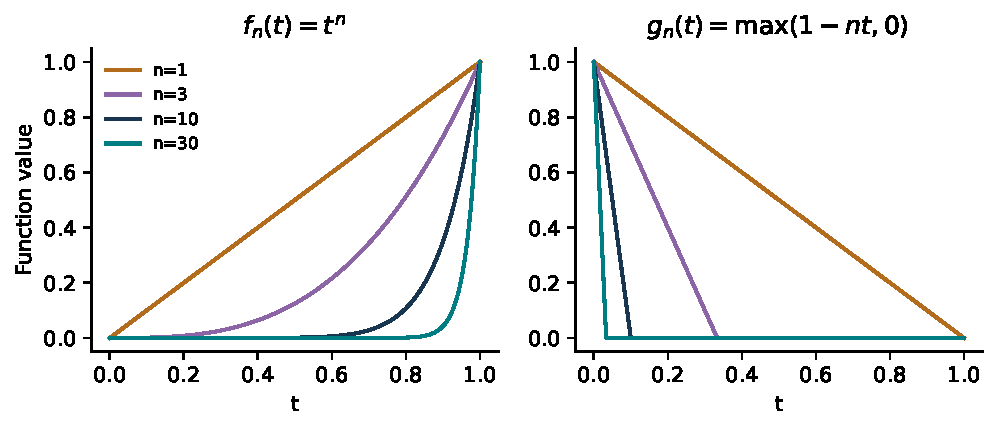
\includegraphics[width=\linewidth]{figures/function_sequences.pdf}\end{center}
On the left, the graphs $t^n$ tend pointwise to zero for $t<1$ but keep the value one at the endpoint. The pointwise limit is discontinuous. On the right, the spikes keep height one while their widths and areas shrink. Thus a small integral error does not force a small supremum error. For the spikes, only convergence in integral distance to zero is asserted; their pointwise limit at zero is one.
\end{note}


\topic{Proof clinic: Why completeness of the function space is not pointwise completeness alone}
\begin{note}{The three obligations in the proof}
A Cauchy sequence $(f_n)$ in a function space is a sequence of whole functions. To prove it converges in that space you need three separate facts:
\begin{enumerate}
\item A candidate function $f$ is defined at every input, usually using completeness of the target at each input.
\item The candidate belongs to the original space: if boundedness or continuity is part of membership, verify it.
\item The distance between $f_n$ and $f$ tends to zero in the specified metric, not merely at each input.
\end{enumerate}
In the sup metric, the uniform Cauchy hypothesis gives one cutoff valid for every input, which is strong enough for the third obligation. The $\varepsilon/3$ continuity proof handles the second obligation for continuous functions. A pointwise limit alone need not satisfy either.
\end{note}
\begin{exam}{Additional practice: diagnose an incomplete argument}
A student writes: ``For each $t$, $f_n(t)$ converges to $f(t)$. Therefore $C([0,1])$ is complete.'' Explain what must be added.
\end{exam}
\begin{answer}
One must begin with an arbitrary sequence Cauchy in the sup metric. The scalar limits define $f$, but it is still necessary to prove $f$ continuous and $\norm{f_n-f}_\infty\to0$. Pass to the limit in the uniform Cauchy bound to obtain uniform convergence. Compare the limit with one bounded term to prove boundedness. Then use uniform convergence and continuity of the approximating functions to show $f$ continuous. Without these steps, the limit might be discontinuous or the convergence might only be pointwise.
\end{answer}


\topic{Proof clinic: Constructing a useful fixed-point domain}
\begin{exam}{Additional practice: the domain makes the theorem usable}
Show $x=(x^2+1)/3$ has exactly one solution in $[0,1]$, but explain why applying the same contraction estimate on all of $\R$ fails.
\end{exam}
\begin{answer}
Let $T(x)=(x^2+1)/3$. On $[0,1]$, $1/3\le T(x)\le2/3$, so $T$ is a self-map. The interval is nonempty and complete. For $x,y\in[0,1]$,
\[|T(x)-T(y)|=\tfrac13|x-y||x+y|\le\tfrac23|x-y|.\]
The constant $2/3<1$ gives a unique fixed point in that interval by Banach. Solving the quadratic gives $x^2-3x+1=0$, so the interval solution is $(3-\sqrt5)/2$; the other root exceeds $1$.

On all of $\R$, the ratio $|T(x)-T(y)|/|x-y|=|x+y|/3$ for distinct points is unbounded, so this map is not globally Lipschitz, much less a strict contraction. The theorem on $[0,1]$ proves uniqueness in that chosen domain, not uniqueness among all real solutions.
\end{answer}
\begin{tip}
Always phrase the conclusion with its domain. A contraction can have only one fixed point in the space to which the theorem is applied; it says nothing about solutions outside that space.
\end{tip}


\topic{Worked lecture exercises}
\exercise{5.1}{Lipschitz maps and completeness}
\begin{exam}{Lecture exercise}
Prove Lipschitz maps preserve Cauchy sequences. Deduce that bi-Lipschitz metric spaces are either both complete or both incomplete.
\end{exam}
\begin{answer}
Suppose $f:E\to F$ satisfies $d_F(fx,fy)\le Ld_E(x,y)$. If $L=0$, $f$ is constant on a nonempty domain and the image of every sequence is constant, hence Cauchy. Assume $L>0$ and let $(x_n)$ be Cauchy in $E$. Given $\varepsilon>0$, choose $N$ such that $d_E(x_n,x_m)<\varepsilon/L$ for $n,m\ge N$. Then
\[d_F(fx_n,fx_m)\le Ld_E(x_n,x_m)<\varepsilon,\]
so the image sequence is Cauchy.

Now let $f$ be a bi-Lipschitz bijection and assume $E$ complete. Given Cauchy $(y_n)$ in $F$, the Lipschitz inverse makes $x_n=f^{-1}(y_n)$ Cauchy in $E$. Hence $x_n\to x\in E$. Since $f$ is Lipschitz and thus continuous, $y_n=f(x_n)\to f(x)\in F$. Thus $F$ is complete. Apply the same argument to $f^{-1}$ for the converse.
\end{answer}
\begin{tip}
For the completeness implication, start with a Cauchy sequence in the space whose completeness you need to prove. Map it to the known complete space, take a limit, and map back.
\end{tip}
\exercise{5.2}{Isometric embedding for an unbounded space}
\begin{exam}{Lecture exercise}
Show that every nonempty metric space embeds isometrically into $\ell^\infty(E;\R)$ using $j_\omega(x)(p)=d(x,p)-d(\omega,p)$ for fixed $\omega\in E$.
\end{exam}
\begin{answer}
First check that each proposed image really is a bounded function of $p$. By reverse triangle inequality,
\[|d(x,p)-d(\omega,p)|\le d(x,\omega)\quad\text{for every }p\in E.\]
The right side depends on the fixed $x$ but not on $p$, so $j_\omega(x)\in\ell^\infty(E;\R)$.

For $x,y,p\in E$, reference terms cancel:
\begin{align*}
|j_\omega(x)(p)-j_\omega(y)(p)|&=|d(x,p)-d(y,p)|\\
&\le d(x,y).
\end{align*}
Taking the supremum over $p$ gives $d_{\sup}(j_\omega(x),j_\omega(y))\le d(x,y)$. At the particular input $p=y$, the absolute difference is $|d(x,y)-d(y,y)|=d(x,y)$. Thus the supremum is also at least $d(x,y)$, proving equality. Hence $j_\omega$ is an isometry.
\end{answer}
\begin{note}{The bound need not be uniform over all image functions}
For membership, each individual function $j_\omega(x)$ must be bounded in its input $p$. There is no requirement for one common bound valid for every $x$. The whole embedded copy may be unbounded, exactly as the original space may be.
\end{note}
\exercise{5.3}{Uniqueness of completion}
\begin{exam}{Lecture exercise; the associated completion proof is marked non-examinable}
For two completions $(\widehat E_1,\iota_1)$ and $(\widehat E_2,\iota_2)$, prove there is exactly one isometry $j:\widehat E_1\to\widehat E_2$ with $j\circ\iota_1=\iota_2$, and show it is onto.
\end{exam}
\begin{answer}
Define $j_0$ on the dense subset $\iota_1(E)$ by $j_0(\iota_1(x))=\iota_2(x)$. This is well-defined because $\iota_1$ is injective. For $x,y\in E$, both embeddings preserve distance, so
\[d_2(j_0\iota_1(x),j_0\iota_1(y))=d_E(x,y)=d_1(\iota_1(x),\iota_1(y)).\]
Thus $j_0$ is isometric. Since its domain is dense and the target completion is complete, the dense Lipschitz-extension theorem gives a unique continuous extension $j$ to $\widehat E_1$, and this extension remains isometric. It satisfies $j\iota_1=\iota_2$ by construction.

To prove surjectivity, let $y\in\widehat E_2$. By density choose $x_n\in E$ with $\iota_2(x_n)\to y$. Then $(x_n)$ is Cauchy in $E$ because $\iota_2$ is isometric. Its images $\iota_1(x_n)$ are Cauchy in complete $\widehat E_1$, so converge to $z$. Continuity of $j$ gives
\[j(z)=\lim_nj(\iota_1(x_n))=\lim_n\iota_2(x_n)=y.\]
Thus $j$ is onto.

Finally any other isometry $k$ satisfying $k\iota_1=\iota_2$ agrees with $j$ on the dense subset $\iota_1(E)$. Isometries are continuous, so the identity theorem implies $k=j$. This proves the precise uniqueness statement.
\end{answer}
\exercise{5.4}{Summably controlled iterates}
\begin{exam}{Lecture exercise}
Suppose $T:E\to E$ on a nonempty complete space satisfies $d(T^nx,T^ny)\le\alpha_nd(x,y)$, where $\alpha_n\ge0$ and $\sum_{n\ge1}\alpha_n<\infty$. Prove Banach's conclusion.
\end{exam}
\begin{method}{Use a contraction iterate, or directly sum consecutive errors}
The summability implies $\alpha_n\to0$, so some iterate has constant below $1$. This gives a short proof. A direct iteration proof also explains the significance of summability.
\end{method}
\begin{answer}
Since $\sum\alpha_n$ converges with nonnegative terms, $\alpha_n\to0$. Choose $K$ with $\alpha_K<1$. Then $T^K$ is a strict contraction on the same nonempty complete space. By the contraction-iterate result, $T$ has one fixed point $p$, and $T^nx\to p$ for every starting point.

For a direct proof, set $x_n=T^nx_0$ and $D=d(x_0,Tx_0)$. For $n\ge1$,
\[d(x_n,x_{n+1})=d(T^nx_0,T^n(Tx_0))\le\alpha_nD.\]
For $m>n\ge1$, triangle inequality gives
\[d(x_n,x_m)\le D\sum_{k=n}^{m-1}\alpha_k\le D\sum_{k=n}^\infty\alpha_k\to0.\]
Thus $(x_n)$ is Cauchy and converges to $p\in E$. The $n=1$ estimate makes $T$ Lipschitz, hence continuous, so $Tp=\lim Tx_n=\lim x_{n+1}=p$. If $p,q$ are fixed, then for every $n$, $d(p,q)\le\alpha_nd(p,q)$; choose $n$ with $\alpha_n<1$ to force $p=q$. This gives existence, uniqueness and convergence.
\end{answer}
\begin{tip}
The nonnegativity of the controlling constants is the natural interpretation of Lipschitz bounds. Summability controls the whole tail, which is stronger than merely having consecutive distances tend to zero.
\end{tip}
\exercise{5.5}{Continuity of a graph parametrisation}
\begin{exam}{Lecture exercise}
For continuous $f:[a,b]\to\R$, prove $F(s)=(f(s),s)$ is continuous into $\R\times[a,b]$.
\end{exam}
\begin{answer}
Use the sum metric $D((u,s),(v,t))=|u-v|+|s-t|$. Fix $s_0\in[a,b]$ and $\varepsilon>0$. Continuity of $f$ at $s_0$ gives $\delta_1>0$ such that $|s-s_0|<\delta_1$ implies $|f(s)-f(s_0)|<\varepsilon/2$. Let $\delta=\min\{\delta_1,\varepsilon/2\}$. Then for $s\in[a,b]$ with $|s-s_0|<\delta$,
\[D(F(s),F(s_0))=|f(s)-f(s_0)|+|s-s_0|<\varepsilon.\]
Thus $F$ is continuous at arbitrary $s_0$. All standard finite-product metrics are equivalent, so the conclusion also holds for the Euclidean product metric.
\end{answer}
\exercise{5.6}{Necessary hypotheses in Cantor intersection}
\begin{exam}{Lecture exercise}
Find counterexamples when shrinking diameters or closedness is removed from Cantor's intersection theorem.
\end{exam}
\begin{answer}
Without shrinking diameters: in complete $\R$, set $F_n=[n,\infty)$. Each set is nonempty and closed; $F_{n+1}\subseteq F_n$. No real number lies in all of them, so the intersection is empty. Their diameters are infinite rather than tending to zero. For failure of uniqueness alone, the constant sequence $F_n=[0,1]$ has non-singleton intersection.

Without closedness: again in complete $\R$, take $F_n=(0,1/n)$. These sets are nonempty and nested with $\diam F_n=1/n\to0$. Their intersection is empty because any positive point is eventually excluded and zero never belongs. They are not closed.

For comparison, if completeness is omitted, take the subspace $E=(0,1)$ and $F_n=(0,1/(n+1)]$. These are closed relative to $E$, nested and shrinking, but have empty intersection. The natural limit zero is missing from $E$.
\end{answer}
\begin{tip}
When a hypothesis is removed, your counterexample must still satisfy all the others. The second example uses a complete ambient space so it isolates closedness as the failing hypothesis.
\end{tip}
\exercise{5.7}{A different Cauchy test and a separated subsequence}
\begin{exam}{Lecture exercise}
(a) Show Cauchyness is equivalent to $\forall\varepsilon>0\ \exists N\ \forall n\ge N:d(x_N,x_n)<\varepsilon$. (b) Show not Cauchy iff some subsequence has consecutive distances with positive infimum.
\end{exam}
\begin{answer}
(a) If Cauchy, choose the usual cutoff $N$ and set one index equal to $N$; the displayed condition follows. Conversely, for a target tolerance $\varepsilon>0$, apply the displayed condition with $\varepsilon/2$, obtaining $N$ with $d(x_N,x_n)<\varepsilon/2$ for all $n\ge N$. For $n,m\ge N$,
\[d(x_n,x_m)\le d(x_n,x_N)+d(x_N,x_m)<\varepsilon.\]
Thus the sequence is Cauchy.

(b) Suppose not Cauchy. Then there is $\eta>0$ such that beyond every cutoff there exist $r,s$ with $d(x_r,x_s)\ge\eta$. Start with any index $n_1$. Having chosen $n_k$, choose $r,s>n_k$ with this separation. At least one of the distances $d(x_{n_k},x_r)$, $d(x_{n_k},x_s)$ is at least $\eta/2$: if both were smaller, triangle inequality would give $d(x_r,x_s)<\eta$. Choose such an index as $n_{k+1}$. This constructs strictly increasing indices with
\[d(x_{n_k},x_{n_{k+1}})\ge\eta/2\quad\text{for every }k.\]
Hence the infimum of these consecutive subsequence distances is positive.

Conversely, if a subsequence has all consecutive distances at least $c>0$, then for every original-sequence cutoff, two sufficiently late selected consecutive terms are at distance at least $c$. This contradicts the Cauchy requirement with $\varepsilon=c$. Thus the original sequence is not Cauchy.
\end{answer}
\begin{note}{What the conclusion does and does not assert}
The proof gives separation between consecutive \emph{subsequence} terms, not necessarily between every pair of selected terms. That is exactly what this exercise requests and is already enough to disprove Cauchyness.
\end{note}
\exercise{5.8}{Optimal Lipschitz constant of integration}
\begin{exam}{Lecture exercise}
On $C([0,1])$ with sup metric, prove $R(f)=\int_0^1f$ is Lipschitz and find $\Lip R$.
\end{exam}
\begin{answer}
For any $f,g$,
\[|R(f)-R(g)|=\left|\int_0^1(f-g)\right|\le\int_0^1|f-g|\le\norm{f-g}_\infty.\]
Thus $1$ is an admissible Lipschitz constant, so $\Lip R\le1$. To prove optimality, choose $f\equiv1$, $g\equiv0$. Then $|R(f)-R(g)|=1$ while $d_{\sup}(f,g)=1$. Their ratio equals $1$, so any admissible constant must be at least $1$. Hence $\Lip R=1$.

On $[a,b]$ the same argument gives optimal constant $b-a$, with constant functions again witnessing equality.
\end{answer}
\exercise{5.9}{Uniformly continuous extension from a dense set}
\begin{exam}{Lecture exercise}
Let $A$ be dense in $E$, $F$ complete, and $f_0:A\to F$ uniformly continuous. Prove there is a unique continuous extension $f:E\to F$ and that it is uniformly continuous.
\end{exam}
\begin{method}{Separate existence, independence and regularity}
First show images of approximating Cauchy sequences converge. Then prove two choices of approximating sequences give the same image limit. Only after the function is well-defined should you prove it extends $f_0$, is uniformly continuous, and is unique.
\end{method}
\begin{answer}
For $x\in E$, density gives a sequence $a_n\in A$ with $a_n\to x$. This is Cauchy. Uniform continuity sends Cauchy sequences to Cauchy sequences: choose its global $\delta$ for a target $\varepsilon$, then use the original Cauchy property for all sufficiently late pairs. Therefore $(f_0(a_n))$ is Cauchy in complete $F$ and has a limit.

If $b_n\in A$ also tends to $x$, then $d_E(a_n,b_n)\le d_E(a_n,x)+d_E(x,b_n)\to0$. Uniform continuity implies $d_F(f_0(a_n),f_0(b_n))\to0$. The two convergent image sequences consequently have the same limit, by continuity of distance. Thus define unambiguously
\[f(x)=\lim_nf_0(a_n).\]
For $x\in A$, take the constant sequence $a_n=x$ to see $f(x)=f_0(x)$.

To prove uniform continuity, fix $\varepsilon>0$. Choose $\eta>0$ such that for $a,b\in A$,
\[d_E(a,b)<\eta\Rightarrow d_F(f_0(a),f_0(b))<\varepsilon/2.\]
Set $\delta=\eta/3$. For any $x,y\in E$ with $d_E(x,y)<\delta$, choose $a_n\to x$, $b_n\to y$ from $A$. Eventually $d_E(a_n,x)<\eta/3$ and $d_E(b_n,y)<\eta/3$, so
\[d_E(a_n,b_n)\le d_E(a_n,x)+d_E(x,y)+d_E(y,b_n)<\eta.\]
Therefore $d_F(f_0(a_n),f_0(b_n))<\varepsilon/2$. Passing to limits yields $d_F(f(x),f(y))\le\varepsilon/2<\varepsilon$. The choice $\delta$ depends only on $\varepsilon$, not on $x,y$, proving uniform continuity.

If $g$ is any continuous extension, then for $a_n\to x$ from $A$,
\[g(x)=\lim_ng(a_n)=\lim_nf_0(a_n)=f(x).\]
Thus $g=f$, proving uniqueness among continuous extensions.
\end{answer}
\begin{tip}
Continuity alone on a dense set need not preserve Cauchy sequences. This is why the uniform-continuity hypothesis is essential to this construction. The target completeness hypothesis is used at the exact point where the image Cauchy sequence needs a limit.
\end{tip}
